\section{Problem}

The Medical test Records project approaches two main problems that hospital information systems must face. \\

The first originates from the sensible information that must be stored in order for the doctors, nurses, assistants... be able to give patients the necessary treatment. A patient profile has associated to it a group of information with different levels of sensibility for example: age, name, blood type, diseases, family records... 
A name is not something sensible so probably most employees can access it, but what about the patient family records? A volunteer has no need to know such information. \\

Given this scenario, the information systems in cause must be able to provide and enforce the correct policies so that different parts of a patient profile are only available to who actually need it and in the correct context. \\

The second problem is in the way that medical tests must be analyzed in different facilities, like partner labs, that are not part of the hospital infrastructure, but require that both are interconnected in a way that enables all sides to identify each other and communicate in a safe and secure way. (Note, in the planning of this project it's assumed that only partner labs with different facilties will realize writes of tests data)\\

\subsection{Requisites}

Given the previous problems, the implementation of this project requires the following security guarantees:
\begin{itemize}
	\item A fine grained access control.
	\item Integrity of all communications with the information systems.
	\item Confidentiality of all communications with the information systems.
	\item Non-repudiation of the tests results data.
	\item Authenticity of the tests results data.
\end{itemize}

\subsection{Trust assumptions}

The main entities in this project are two, the hospital information system and the clients that try to access said system. \\

The client entity can be internal or external to the hospital infrastructure, if the context is internal, the client is used by the hospital staff (doctors, nurses...). In case the client is used by the partner labs to send the tests data result, the client is external. \\

In both cases the client is untrusted, the information systems will require some type of authentication and authorization before the request is accepted. \\ 

There is also a full trust assumption, that the code responsible for the access control is error free and an unauthorized person will never be able to access something is not supposed. \\

\section{Proposed solution}

The implementation will be separated in two main components, a REST API and a client of the API.
All communications from the client to the API (and vice-versa) will run with TLS to provide confidentiality, integrity and freshness. TLS will be provided by the Spring framework, which will be used to develop the API. \\

	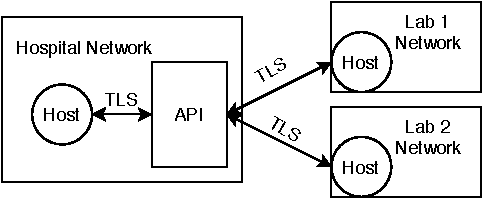
\includegraphics[width=.4\textwidth]{figs/network_layout.pdf}
	
TLS will require the definition of a couple certificates, the Hospital certificate to actually create the TLS tunnel and the laboratory certificates (each lab will have its own certificate), which will be used to digitally sign the sent data (non-repudiation and authenticity). \\ 

All requests received by the API need to posess a proof of identity to be further processed (accept or refuse action), in this case will be a token provided by the API after authentication using the correct set of credentials (username:password). The token is transported in the "Authorization" header of the HTTP request. If the token is not present the request will be refused with status code 401 UNAUTHENTICATED. \\

If the request contains all necessary information (token), it will be forwarded to the access control mechanism. \\

The access control mechanism is composed by 4 major components:
\begin{itemize}
	\item PEP - Policy Enforcement Point
	\item PDP - Policy Decision Point
	\item PAP - Policy Administration Point
	\item Policy Store
\end{itemize}

The PEP will send a XACML request to the PDP, the PDP will then based on the policies defined by the system return a XACML response which will dictate the action (ACCEPT or REFUSE) that PEP will enforce. If the result is ACCEPT, the request will continue and read or write the requested resource, otherwise the request will be dropped and replied with a 403 UNAUTHORIZED.

	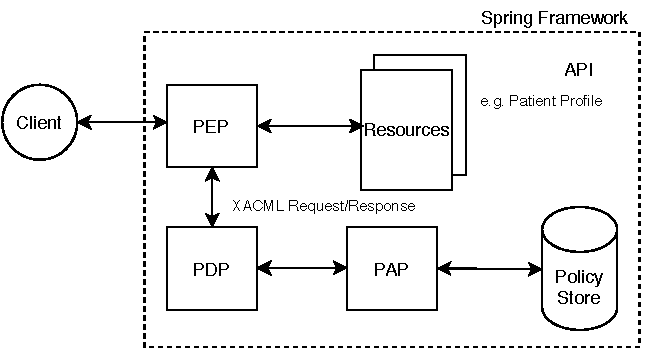
\includegraphics[width=.6\textwidth]{figs/access_control.pdf}
	
	
Example of client utilization: \\
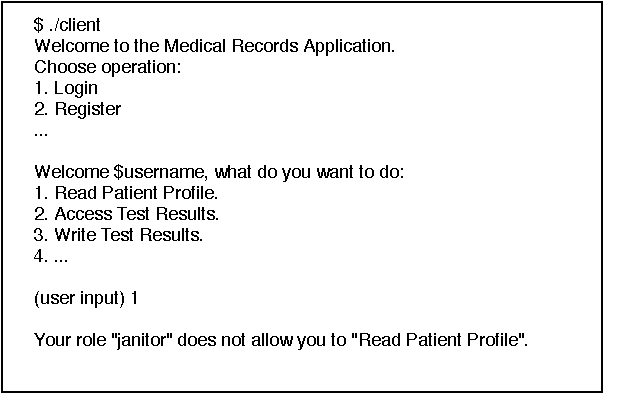
\includegraphics[width=.6\textwidth]{figs/client_utilization.pdf}


\section{Plan}

\subsection{Basic}
The basic version of the project must have the following components in place:
\begin{itemize}
	\item API
	\item Client
	\item TLS for secure communication channels
	\item Access Control
\end{itemize}

It is expected that this version will take around 2 weeks to complete (worst case scenario). 


\subsection{Intermediate}
The intermediate version will expand what was built in the first 2 weeks adding the following:
\begin{itemize}
	\item The necessary mechanism to check tests data authenticity at any time. (Digital Signature)
	\item Partner Labs TLS Muthual Authentication. (To guarantee the information systems will only accept communications from trusted sources, in the previous case an attacker with stolen credentials could send false data, the downside is that now also the hosts in the hospital network will need a certificate). 
	\item Correcting any bugs left in the access control
\end{itemize}

This phase should take around 1 week.


\subsection{Advanced}

By this point the necessary mechanisms are all implemented, possible bugs should be corrected now, if there are none, the project can take a step further and do the following to increment the security or optimize the system:

\begin{itemize}
	\item Policies and authentication information cache. (Will avoid constant reads to the database everytime there is a request)
	\item Defining rule combining algorithms in the access control for  more complex decisions.
	\item Firewall implementation.
\end{itemize}


\subsection{Effort Commitment}

\begin{tabularx}{0.8\textwidth} { 
  | >{\centering\arraybackslash}X 
  | >{\centering\arraybackslash}X 
  | >{\centering\arraybackslash}X 
  | >{\centering\arraybackslash}X | }
 \hline
  & Alexandru & Ana  & Rafaela \\
 \hline
 Week 1  & API and Access Control  & Deployment Scripts and Client  & Database and Client \\
  \hline
  Week 2  & TLS and management of certificates  & Authenticity Mechanism client adaptation  & Authenticity Mechanism database adaptation \\
   \hline
   Week 3  & TLS Mutual Authentication  & Authenticity Mechanism  & Authenticity Mechanism \\
    \hline
    Week 4  & Firewall  & Rule Combining Algorithms  & Optimizations \\
\hline
\end{tabularx}

\section{References}

The project client and API infrastructure will be developed using the Java programming language. \\

The API will use the \href{https://docs.spring.io/spring-framework/docs/3.2.x/spring-framework-reference/html/mvc.html}{Spring Web MVC} Framework to attend and process the client requests, enable the TLS communications and manage the KeyStores (own certificate) and TrustStores (partner labs certificates). \\

The deployment scripts will use \href{https://www.vagrantup.com/}{Vagrant} to manage and deploy the VM's with the correct network configurations and all the necessary software to run the applications. \\

The database management system will be provided by \href{https://www.mysql.com/}{MySQL}. \\

Finally, the certificates will be self-signed and created using \href{https://www.openssl.org/}{OpenSSL}.
